\documentclass[tikz,border=2pt,png]{standalone}
\usepackage{tkz-euclide}
\usetkzobj{all}

\begin{document}
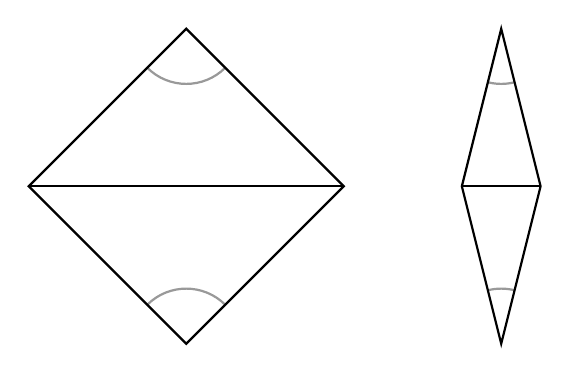
\begin{tikzpicture}[thick]
\coordinate (T0) at (0.0,0);
\coordinate (T1) at (4,0);
\coordinate (T2) at (2.0,2);
\coordinate (T3) at (2.0,-2);

\draw (T2)--(T0)--(T3)--(T1)--cycle;

\draw (T0)--(T1);

\tkzMarkAngle[fill=gray,size=0.7cm,%
opacity=.4](T0,T2,T1)

\tkzMarkAngle[fill=gray,size=0.7cm,%
opacity=.4](T1,T3,T0)


\coordinate (S0) at (5.5,0);
\coordinate (S1) at (6.5,0);
\coordinate (S2) at (6.0,2);
\coordinate (S3) at (6.0,-2);

\draw (S2)--(S0)--(S3)--(S1)--cycle;

\draw (S0)--(S1);

\tkzMarkAngle[fill=gray,size=0.7cm,%
opacity=.4](S0,S2,S1)

\tkzMarkAngle[fill=gray,size=0.7cm,%
opacity=.4](S1,S3,S0)

\end{tikzpicture}
\end{document}